\documentclass[letterpaper, 10 pt, conference]{ieeeconf}

\IEEEoverridecommandlockouts

\overrideIEEEmargins

\usepackage{graphics} % for pdf, bitmapped graphics files
\usepackage{epsfig}
\usepackage{amsmath} % for postscript graphics files
\usepackage{subfigure}
\usepackage{fullpage}

\graphicspath{{../figures/}}

\title{\LARGE \bf
  Vision Based Obstacle Avoidance Using Neuro-Evolutionobot in Simulation
}

\author{Devin Koepl, Kevin Kemper}

\begin{document}
	\maketitle

	\begin{abstract}

		In this proposal we present our idea for using a collection of compact neural networks for vision based obstacle avoidance on a simple robot in simulation. Our approach uses many simple neural networks working in concert to select a heading at each time step based on the networks' confidence that the path chosen is clear.  We believe that a collection of simple networks will be capable of better performance than any simple reflex controller we find and of similar performance to a single large neural network provided sufficient training time, but will converge to a good solution faster than the large network.

	\end{abstract}

	\section*{INTRODUCTION}

		Neural networks are convenient for problem spaces with many inputs, and are often applied to machine vision problems were each pixel acts as one or more inputs to the network \cite{Pomerleau93_NNforVehicles},\cite{EgmontPetersen2002imageprocessingNN}.  Current cameras have millions of color pixels, for a neural network to make full use of this type of resolution it needs one or more inputs for each of the camera's pixels and perhaps thousands of hidden units.  Training and utilizing very large neural networks can be difficult because computations become expensive for the large number of training examples required to train them. The training examples also increases in complexity for neural networks with large numbers of inputs, and training time increases for online learning. Conventional techniques use low resolution cameras or pre-processing algorithms to limit the complexity of neural networks and shorten training.

		Our proposed approach will use a collection of simple neural networks that will be easier to train than a single large network, and will collectively be able to avoid obstacles as well as the large network.  Instead of identifying and avoiding hazards in an entire image, each of our neural networks will only need to output an approximation of how safe it is to precede in the direction it is provided as a narrow column of the pre-processed image.  As an added benefit, we will be able to reuse the same collection of neural networks on all of the available directions, because the narrow columns that the pre-processed image is divided into are identical in size, reducing the amount of information that has to be stored.


		\begin{figure}
			\begin{center}
				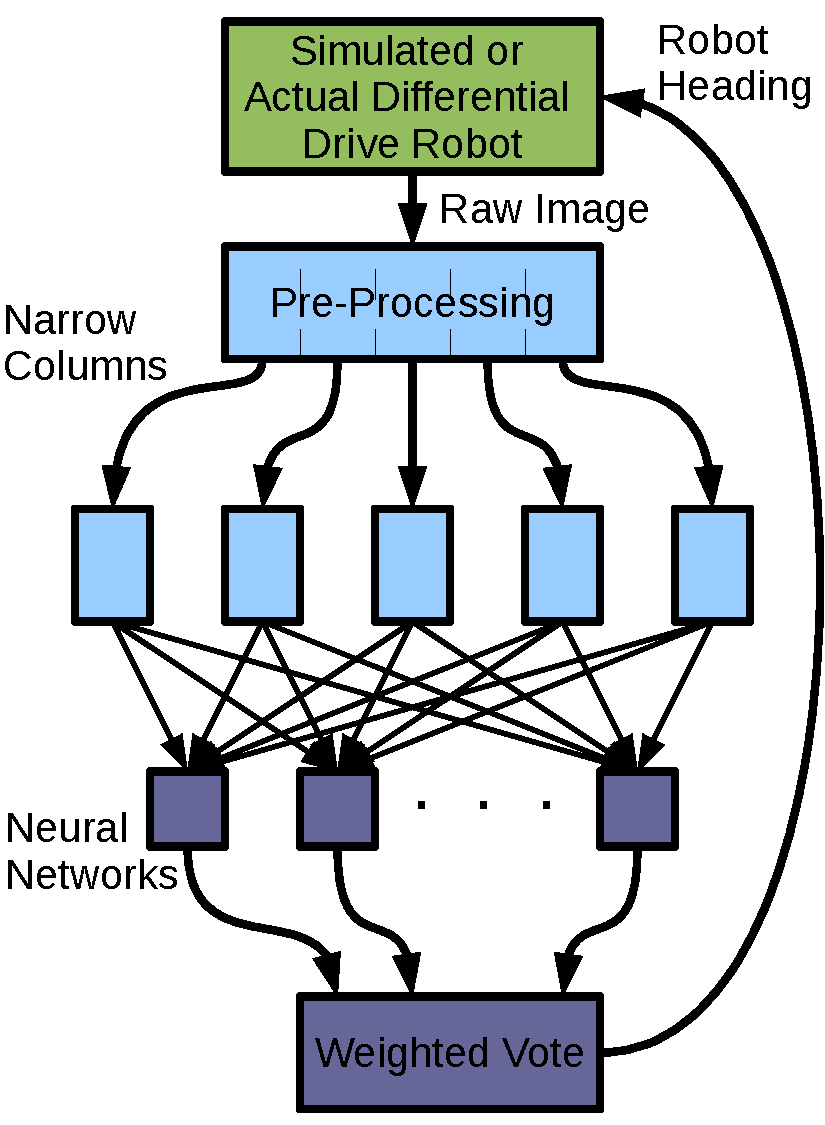
\includegraphics[width=\columnwidth]{block_diagram.pdf}
			\end{center}
			\caption{Block diagram of the neural network solution we will create.}
			\label{block_diagram}
		\end{figure}

	\section*{BACKGROUND}

		
		In \cite{Baluja97visionbasedfocus} paper has presented a method for dynamic relevance assessment using artificial neural networks. The network’s allocation of its limited representation capacity at the hidden layer is an indicator of what inputs it deems relevant to the task. By using only the hidden layer to predict the next input image, and comparing this prediction with the actual next image, they show that it is possible to estimate which inputs should be ignored and which should be attended. In deciding whether this approach is suitable to a new problem, there are two main criteria that must be considered. First, if expectation is to be used to remove distractions from the inputs, then given the current inputs, the activations of the relevant inputs in the next time step must be predictable. Additionally, the irrelevant inputs must either be unrelated to the task or be unpredictable.
		Nelson argued that the flow field divergence represents a qualitative measurement which is useful for obstacle avoidance during visual navigation \cite{Nelson89ObstacleAvoidanceFlow}.  Coombs demonstrated a system that uses only real-time motion cues to wander while avoiding obstacles in a laboratory containing office furniture and robot and computing equipment \cite{Coombs98obstacleavoidanceflow}. The paper describes how flow, divergence of flow, and maximal flows are computed in real-time to provide the robot’s sense of space, and how steering, collision detection, and camera gaze control together accomplish safe wandering.
		ALVINN (Autonomous Land Vehicle In A Neural Network)\cite{Pomerleau93ALVINN} is the neural network based lane-keeping system. Using simple color image preprocessing to create a cigrayscale input image and a 3 layer neural network architecture, ALVINN can learn, using back-propagation, the correct mapping from input image to output road location. This steering direction is used to control our testbed vehicle, a converted U.S. Army HMMWV called the Navlab 2. On this vehicle, ALVINN has driven at speeds up to 55 m.p.h. for 90 continuous miles \cite{Jochem95visionbasedNNroaddetection}.
		An interesting aspect of the ALVINN system is the method used to train it \cite{Pomerleau93_NNforVehicles}.  In this technique, called training "on-the-fly" the network is taught to imitate the driving reactions of a person.  As a person drives, the network is trained with back propagation using the latest video image as input the person's steering direction as the desired output.

	\section*{PROBLEM DOMAIN}

		Our proposed approach will use a pool of simple, single-layer neural networks that accept a narrow column of the pre-processed image captured by our robot's camera and return a confidence that the small image represents a safe direction to precede in, as shown in Fig. \ref{block_diagram}.  At each time step an image will be captured by our robot's camera, such as the image shown in Fig. \ref{input}, but from simulation, and not from the real world for now, and our robot's heading will be chosen by a weighted vote between the neural networks.  Each neural network will be used on each column of the pre-processed image, and will cast a vote based on its confidences in each of the directions represented by the columns, with a weight reflective of its accuracy during training.

		Our approach will use online neuro-evolution techniques to create a collection of neural networks capable of navigating the simulated robot through its environment while colliding with as few obstacles as possible.  Training will begin with a collection of neural networks with random weights and uniform voting power, and will consist of releasing the simulated robot in a training environment.  Large penalties will be assessed after collisions with the environment based on networks' confidences in the direction that led to the collision, and smaller penalties will be assessed to the neural networks that expressed confidence in the directions that led up to the collision.  Rewards will be given for confidence in directions that do not lead to collisions.  We would also like to investigate more omniscience rewards that consider our robot's proximity to hazards and assess rewards for maintaining its distance from hazards.  After each timestep, the poorest performing neural networks will be discarded, and the best performing neural networks will be duplicated with some mutations and an initial voting power that places them in the lower-middle of the collection, maintaining the size of the neural network collection. 

		We will use Open Dynamics Engine (ODE) to simulate our robot in its environment.  ODE will handle any physics that are required and any collisions that occur between our robot and the environment.  In addition to ODE we will also use Robot Operating System (ROS).  ROS includes a 3D visualization environment RVIZ, which we will use to generate and capture images for input into our controller.  We will use OpenCV for our pre-processing routine, as this library includes functions for edge and flow detection, as shown in Fig. \ref{output}.  The controllers we will compare in this paper will be implemented in C++ such that they can be easily compiled into a program that includes the ODE and RVIZ libraries, or compiled as standalone executables that communicate with the physics simulation and visualization using ROS.  In addition to RVIZ, ROS also includes methods for linking independent processes running on a single machine using shared memory.  While we may choose to simply compile the ODE and ROS libraries into our simulation, we also have the option to link our physics simulation, visualization, and controllers using ROS topics. 

		Our robot will travel at a constant speed, and will not be able to adjust its speed, it will only be able to control its heading.  Although our robot's environment will be continuous, it will only be able to update its heading at regular fixed timestep intervals.  This simulates the hardware limitations of a mobile robot driving in the real world, where image capture and computation are not instantaneous.

	\begin{figure}
		\subfigure[Raw input image captured from a standard webcam that could be used on a small mobile robot.  Eventually images will be captured from our simulation.]{
			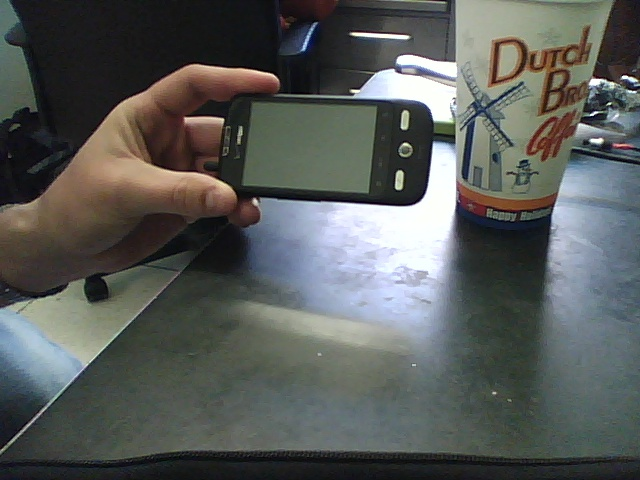
\includegraphics[width=0.46\columnwidth]{input.jpg}
			\label{input}
		}
		\subfigure[Pre-processed image with Canny edge (white lines) and optical flow detection (color squares).  Blue squares represent lower absolute velocities and red squares represent higher absolute velocities.]{
			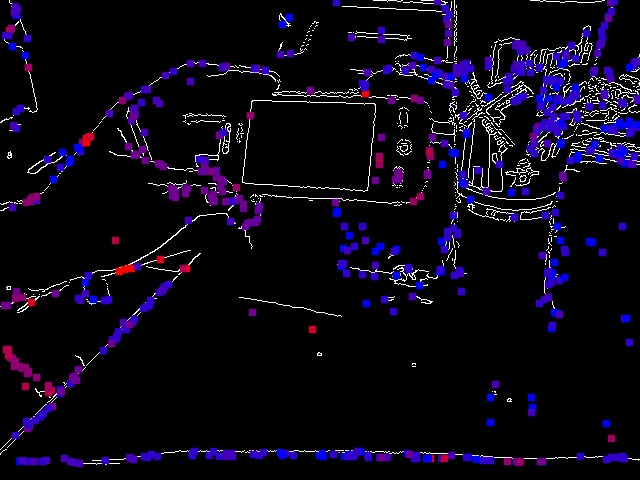
\includegraphics[width=0.46\columnwidth]{output.jpg}
			\label{output}
		}
		\caption{Example pre-processing of a test image captured from a webcam.}
	\end{figure}


	\section*{PROBLEM DOMAIN}

		Our proposed approach will use a pool of simple, single-layer neural networks that accept a narrow column of the pre-processed image captured by our robot's camera and return a confidence that the small image represents a safe direction to precede in, as shown in Fig. \ref{block_diagram}.  At each time step an image will be captured by our robot's camera and the direction the robot travels in will be chosen by a weighted vote between the neural networks.  Each neural network will be used on each column of the pre-processed image, and will cast a vote based on its confidences in each of the directions represented by the columns, with a weight reflective of its accuracy during training.

		Our approach will use online neuro-evolution techniques to create a collection of neural networks capapble of navigating the simulated robot through its environment while colliding with as few obstacles as possible.  Training will begin with a collection of neural networks with random weights and uniform voting power, and will consist of releasing the simulated robot in a training environment.  Large penalties will be assessed after collisions with the environment based on networks' confidences in the direction that led to the collision, and smaller penalties will be assessed to the neural networks that expressed confidence in the directions that led up to the collision.  Rewards will be given for confidence in directions that do not lead to collisions.  We would also like to investigate more omnipitent rewards that consider our robot's proximity to harzards and assess rewards for maintaining its distance from hazards.  After each timestep, the poorest performing neural networks will be discarded, and the best performing neural networks will be duplicated with some mutations and an initial voting power that places them in the lower-middle of the collection, maintraining the size of the neural network collection. 

		We will use Open Dynamics Engine (ODE) to simulate our robot in its environment.  ODE will handle any physics that are required and any collisions that occur between our robot and the environment.  In addition to ODE we will also use Robot Operating System (ROS).  ROS includes a 3D visualization environment RVIZ, which we will use to generate and capture images for input into our controller.  We will use OpenCV for the pre-processing shown in Fig. \ref{output}, this libarary includes the edge and flow detection algorithms we will use in our pre-processing routine. The controllers we will compare in this paper will be implemented in C++ such that they can be easily compiled into a program that includes the OpenCV, ODE, and RVIZ libraries, or compiled as standalone executables that include OpenCV, but communicate with the physics simulation and visualization using ROS.  In addition to RVIZ, ROS also includes methods for linking independent processes running on a single machine using shared memory.  While we may choose to simply compile the ODE and ROS libaries into our simulation, we also have the option to link our physics simulation, visualization, and controllers using ROS topics. 

		Our robot will travel at a constant speed, and will not be able to adjust its speed, it will only be able to control its heading.  Although our robot's environment will be continuous, it will only be able to update its heading at regular fixed timestep intervals.  This simulates the hardware limitations of a mobile robot driving in the real world, where image capture and computation are not instantaneous.

	\section*{EXPERIMENTS}

		We will compare our collective neural network approach to a single neural network solution and controllers that we devise in simulation.  We will generate a training environment, and several test environments with varying levels of complexity which we will simulate in ODE.  We will plot performance versus the number of training epochs for the controllers in several test environments.  Performance will be measured as the probability that a collision occurs during a timestep in a test environment.  This measurement will be taken by setting a robot loose in the environment for a large fixed number of timesteps.  When a collision occurs the robot will be reset to a random position in the environment.  After all of the timesteps are completed the probability that a collision occurs in a timestep is just the total number of collisions that occurred divided by the length of the test.

		We will compare our neural network solutions against simple reflex agent controllers of our own design.  These controllers will include a controller that directs our robot to drive in the direction of the lowest absolute optical flows, a controller that directs our robot to drive in the direction of the fewest edges, and any other controllers that we find to test against.  We suspect that the single and collective neural network solutions will be able to outperform any simple reflex agent we devise to control our robot, given sufficient training time.  The simple reflex agents will be able to avoid obstacles in specific environments, but will not be able to avoid obstacles in other environments.  For example, the simple reflex agent that drives towards lower concentrations of edges will perform poorly in environments with a textured ground surface and smooth solid colored objects.

		If time allows we would like to investigate different reward structures and pre-processing algorithms.  We believe that the performance of either a single neural network solution or our collective neural network solution could be improved by giving rewards for increasing the distance between our robot and obstacles in the environment and assessing penalties for coming close to colliding.  In addition to our edge and flow detection algorithms, we would also like to test other algorithms as part of our pre-processing routine.  For example, we suspect that we can improve the performance of either of the neural network controllers we are testing by averaging several successive images together at each time step.

	\bibliographystyle{plain}
	\bibliography{../papers/me537.bib}

\end{document}
